\documentclass[12pt]{article}
\usepackage[brazil]{babel}
\usepackage[utf8]{inputenc}
\usepackage[T1]{fontenc}
\usepackage{amsmath, amssymb}
\usepackage{geometry}
\usepackage{graphicx}
\usepackage{tikz}
\usetikzlibrary{shapes,arrows}
\usepackage{xcolor}
\usepackage{enumitem}
\usepackage{caption}
\usepackage{float}
\usepackage{listings}

% Configuração para listagem de código
\definecolor{codegreen}{rgb}{0,0.6,0}
\definecolor{codegray}{rgb}{0.5,0.5,0.5}
\definecolor{codepurple}{rgb}{0.58,0,0.82}
\definecolor{backcolour}{rgb}{0.95,0.95,0.92}

\lstset{
    backgroundcolor=\color{backcolour},   
    commentstyle=\color{codegreen},
    keywordstyle=\color{magenta},
    numberstyle=\tiny\color{codegray},
    stringstyle=\color{codepurple},
    basicstyle=\ttfamily\small,
    breakatwhitespace=false,         
    breaklines=true,                 
    captionpos=b,                    
    keepspaces=true,                 
    numbers=left,                    
    numbersep=5pt,                  
    showspaces=false,                
    showstringspaces=false,
    showtabs=false,                  
    tabsize=2,
    language=C++
}

\definecolor{maincolor}{RGB}{0,100,50}
\usepackage{fancyhdr}
\definecolor{forestgreen}{RGB}{0,100,50}
\usepackage[most]{tcolorbox}

\newtcolorbox{block}[1]{%
  colback=green!5,
  colframe=maincolor,
  coltitle=white, 
  title=#1,
  fonttitle=\bfseries,
  boxrule=1.5pt,
  arc=3mm,
  left=6pt,
  right=6pt,
  top=6pt,
  bottom=6pt
}

\geometry{margin=2.5cm}
\pagestyle{fancy}
\fancyhf{}

\renewcommand{\headrulewidth}{2pt}
\renewcommand{\footrulewidth}{2pt}

\renewcommand{\headrule}{\hbox to\headwidth{%
  \color{forestgreen}\leaders\hrule height \headrulewidth\hfill}}

\renewcommand{\footrule}{\hbox to\headwidth{%
  \color{forestgreen}\leaders\hrule height \footrulewidth\hfill}}

\setlength{\headheight}{51pt}

\fancyhead[L]{%
  
\includegraphics[height=1.2cm]{Universidade_de_Rio_Verde.jpg}
}

\fancyhead[R]{%
  \raggedleft
  \textcolor{forestgreen}{%
    \small
    \textbf{Lista de Exercícios — Problemas de Eletrônica}\\
    Me.~Sergio Souza Novak\\
    \textit{Lógica para Engenharia de Software}
  } 
}

\fancyfoot[C]{%
  \textcolor{forestgreen}{\thepage}
}

\begin{document}

\vspace*{0.2cm}

% ──────────────────────────────────────────────────────────────────────────────
\subsection*{Exercício 1 — Sistema Inteligente de Liberação para Ordenha}

Diversos estudos científicos, tanto no Brasil quanto no exterior, têm investigado o uso de sistemas inteligentes de liberação para ordenha baseados em Internet das Coisas (IoT), com ênfase na aplicação de sensores como RFID, monitoramento da atividade ruminal, detecção de presença e avaliação da saúde animal para automatizar o controle de acesso. No contexto brasileiro, pesquisas recentes apontam avanços significativos na adoção dessas tecnologias. Um levantamento da Embrapa, realizado em 2024, analisou 73 fazendas equipadas com 143 robôs de ordenha e destacou que cerca de 70,7% operam em regime de tráfego livre, no qual as vacas são liberadas voluntariamente após identificação por RFID e monitoramento de suas condições, evidenciando um modelo semelhante ao de sistemas inteligentes de aptidão. Outro estudo, conduzido pela Unijuí, avaliou a eficiência de sistemas de ordenha robotizada em ambientes freestall no Rio Grande do Sul, utilizando sensores de presença e identificação para mensurar taxas de recusa e a eficiência do fluxo automatizado de liberação.

No campo acadêmico, pesquisas sobre IoT aplicada à pecuária reforçam a relevância desses sistemas. Um estudo publicado em 2024 aborda os sistemas automáticos de ordenha (AMS), destacando o uso de sensores como SCR Heatime, voltado ao monitoramento de atividade, CowManager, que avalia parâmetros de saúde e temperatura, e o RFID Allflex, empregado na identificação animal, permitindo decisões mais precisas.
Em um piquete de vacas leiteiras, um sistema automatizado decide se uma vaca
pode entrar na área de ordenha com base em sensores IoT industriais.
Os quatro sensores utilizados são:

\begin{itemize}[leftmargin=1cm, label=\textbullet]
  \item \textbf{A} — Sensor RFID de identificação animal (\textit{Allflex Livestock Intelligence}):\\
        $A = 1$ indica que a vaca foi identificada corretamente.
        \begin{figure}[H]
          \centering
          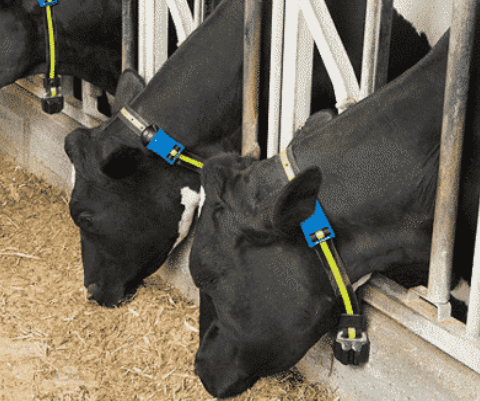
\includegraphics[width=4cm]{Allflex.png}
          \caption{Sensor RFID Allflex Livestock Intelligence.}
          \label{fig:allflex}
        \end{figure}

  \item \textbf{B} — Sensor de atividade/ruminação (\textit{SCR Heatime HR Tag}):\\
        $B = 1$ indica atividade normal (vaca apta).
        \begin{figure}[H]
          \centering
          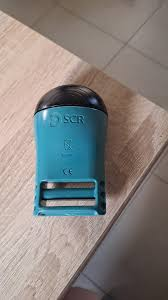
\includegraphics[width=4cm]{SCR Heatime HR Tag1.jpeg}
          \caption{Sensor de atividade/ruminação SCR Heatime HR Tag.}
          \label{fig:scr_heatime}
        \end{figure}

  \item \textbf{C} — Sensor de presença no portão (\textit{sensor indutivo IFM Efector}):\\
        $C = 1$ indica que a vaca está posicionada corretamente no portão.
        \begin{figure}[H]
          \centering
          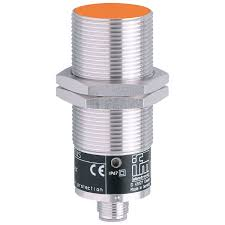
\includegraphics[width=4cm]{ensor indutivo IFM Efector .jpeg}
          \caption{Sensor indutivo de presença IFM Efector.}
          \label{fig:ifm_efector}
        \end{figure}

  \item \textbf{D} — Sensor de saúde — temperatura corporal (\textit{CowManager Sensor}):\\
        $D = 1$ indica temperatura corporal normal.
        \begin{figure}[H]
          \centering
          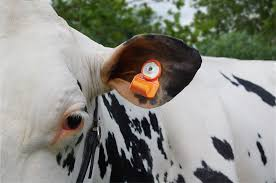
\includegraphics[width=4cm]{CowManager Sensor.jpeg}
          \caption{Sensor de saúde CowManager.}
          \label{fig:cowmanager}
        \end{figure}
\end{itemize}

\medskip

\medskip
\textbf{Saída do sistema:} $Y = 1$ libera a entrada para a ordenha;
$Y = 0$ não libera.

\bigskip

\noindent\textbf{Tabela Verdade:}

\medskip
\begin{center}
\renewcommand{\arraystretch}{1.25}
\begin{tabular}{|c|c|c|c||c|}
  \hline
  \textbf{A} & \textbf{B} & \textbf{C} & \textbf{D} & \textbf{Y} \\
  \hline
  0 & 0 & 0 & 0 & 0 \\
  0 & 0 & 0 & 1 & 1 \\
  0 & 0 & 1 & 0 & 0 \\
  0 & 0 & 1 & 1 & 0 \\
  0 & 1 & 0 & 0 & 1 \\
  0 & 1 & 0 & 1 & 0 \\
  0 & 1 & 1 & 0 & 0 \\
  0 & 1 & 1 & 1 & 0 \\
  1 & 0 & 0 & 0 & 0 \\
  1 & 0 & 0 & 1 & 0 \\
  1 & 0 & 1 & 0 & 1 \\
  1 & 0 & 1 & 1 & 0 \\
  1 & 1 & 0 & 0 & 0 \\
  1 & 1 & 0 & 1 & 0 \\
  1 & 1 & 1 & 0 & 0 \\
  1 & 1 & 1 & 1 & 1 \\
  \hline
\end{tabular}
\end{center}

\bigskip

\noindent\textbf{O que você deve fazer:}

\begin{enumerate}[label=\textbf{\alph*)}, leftmargin=2cm]
  \item Escreva a função booleana na forma \textbf{Soma de Produtos (SOP)} canônica,
        identificando os mintermos com saída $Y = 1$.
  \item Simplifique a expressão obtida usando apenas \textbf{Álgebra Booleana}
        (sem utilizar mapa de Karnaugh), apresentando cada passo da simplificação
        com a propriedade ou lei aplicada.
  \item Construa o circuíto de portas lógicas para esse sistema.
\end{enumerate}
\newpage
\subsection*{Exercício 2 — Controle de Irrigação com Estação Meteorológica}
Manejo automatizado baseado em dados meteorológicos é um tipo de manejo consolidado como uma das principais inovações da agricultura de precisão, permitindo decisões mais eficientes e sustentáveis no manejo hídrico. Nesse modelo, sensores instalados em estações meteorológicas — como pluviômetros, anemômetros, higrômetros e piranômetros — realizam a coleta contínua de informações sobre precipitação, velocidade do vento, umidade relativa do ar e radiação solar. Esses dados são processados em tempo real por algoritmos agrometeorológicos que calculam a evapotranspiração de referência (ETo), geralmente por meio do método de Penman-Monteith, amplamente reconhecido como padrão internacional \cite{allen1998}. A partir desse cálculo, o sistema determina a lâmina de irrigação ideal, ajustando automaticamente a quantidade de água aplicada conforme a necessidade das culturas.

A automação do processo ocorre por meio de um controlador central, que pode ser um Controlador Lógico Programável (CLP) ou um microcontrolador, como o ESP32. Esse dispositivo recebe as informações dos sensores, processa os dados e aciona válvulas solenoides responsáveis pela liberação de água em diferentes setores da área cultivada. Esse controle setorizado permite otimizar parâmetros hidráulicos como pressão e vazão, além de reduzir desperdícios. No Brasil, soluções desse tipo já são realidade em sistemas de irrigação inteligente, que utilizam tecnologias de Internet das Coisas (IoT) para monitoramento remoto via aplicativos e plataformas digitais. Estudos indicam que a adoção dessas tecnologias pode reduzir o consumo de água em até 30\% em sistemas de pivô central \cite{bassoi2024}.

Além dos ganhos operacionais, os benefícios práticos desse tipo de sistema são expressivos. A substituição de decisões baseadas exclusivamente na experiência do produtor por estratégias orientadas a dados contribui para o aumento da eficiência hídrica, da produtividade e da sustentabilidade agrícola. Instituições de pesquisa como a Embrapa têm desenvolvido e validado protótipos que integram sensores meteorológicos ao manejo de culturas como soja e milho, especialmente em regiões do Centro-Oeste brasileiro, onde a gestão racional da água é cada vez mais crítica. Paralelamente, o avanço das tecnologias baseadas em IoT no setor agropecuário reforça o potencial desses sistemas, como destacado por Tangorra et al. \cite{tangorra2024}, ao evidenciar a capacidade dos sensores inteligentes em otimizar processos produtivos e promover maior controle operacional no campo.

\bibliographystyle{plain}
\begin{thebibliography}{9}

\bibitem{allen1998}
ALLEN, R. G.; PEREIRA, L. S.; RAES, D.; SMITH, M.
\textit{Crop evapotranspiration: Guidelines for computing crop water requirements}.
Rome: FAO, 1998.

\bibitem{bassoi2024}
BASSOI, L. H. et al. (ed.).
\textit{Agricultura de precisão: um novo olhar na era digital}.
São Carlos: Cubo, 2024.

\bibitem{tangorra2024}
TANGORRA, F. M.; BUOIO, E.; CALCANTE, A.; BASSI, A.; COSTA, A.
Internet of Things (IoT): Sensors Application in Dairy Cattle Farming.
\textit{Animals}, v. 14, n. 21, p. 3071, 2024. DOI: 10.3390/ani14213071.

\end{thebibliography}
\textbf{Contexto.}
Um sistema de irrigação automatizado utiliza sensores de uma estação meteorológica
para definir a lâmina de irrigação e acionar válvulas solenoides.

\textbf{Entradas (Sensores):}

\begin{itemize}[leftmargin=1.5cm, label=\textbullet]
  \item \textbf{T} — Temperatura alta ($1 = $ acima do ideal).
  \item \textbf{U} — Umidade do ar baixa ($1 = $ ar seco).
  \item \textbf{S} — Umidade do solo baixa ($1 = $ solo seco).
  \item \textbf{R} — Chuva detectada ($1 = $ está chovendo).
\end{itemize}

\textbf{Saídas:}

\begin{itemize}[leftmargin=1cm, label=\textbullet]
  \item \textbf{A, B, C, D} — Válvulas solenoides de irrigação (abertura proporcional de 25\%, 50\%, 75\% e 100\%).
        \begin{figure}[H]
          \centering
          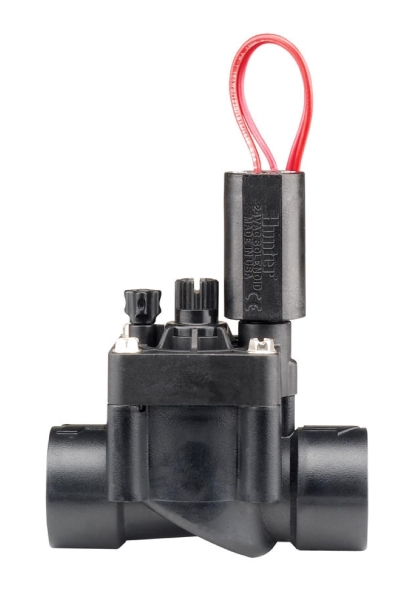
\includegraphics[width=4cm]{solenoide.jpg}
          \caption{Válvula solenoide de irrigação.}
          \label{fig:solenoide}
        \end{figure}

  \item \textbf{P} — Bomba hidráulica de alta pressão para alimentação do sistema.
        \begin{figure}[H]
          \centering
          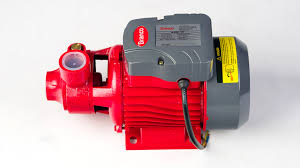
\includegraphics[width=4cm]{bomba_hidraulica.jpeg}
          \caption{Bomba hidráulica de alta pressão.}
          \label{fig:bomba_hidraulica}
        \end{figure}
\end{itemize}
 
\begin{figure}[H]
  \centering
  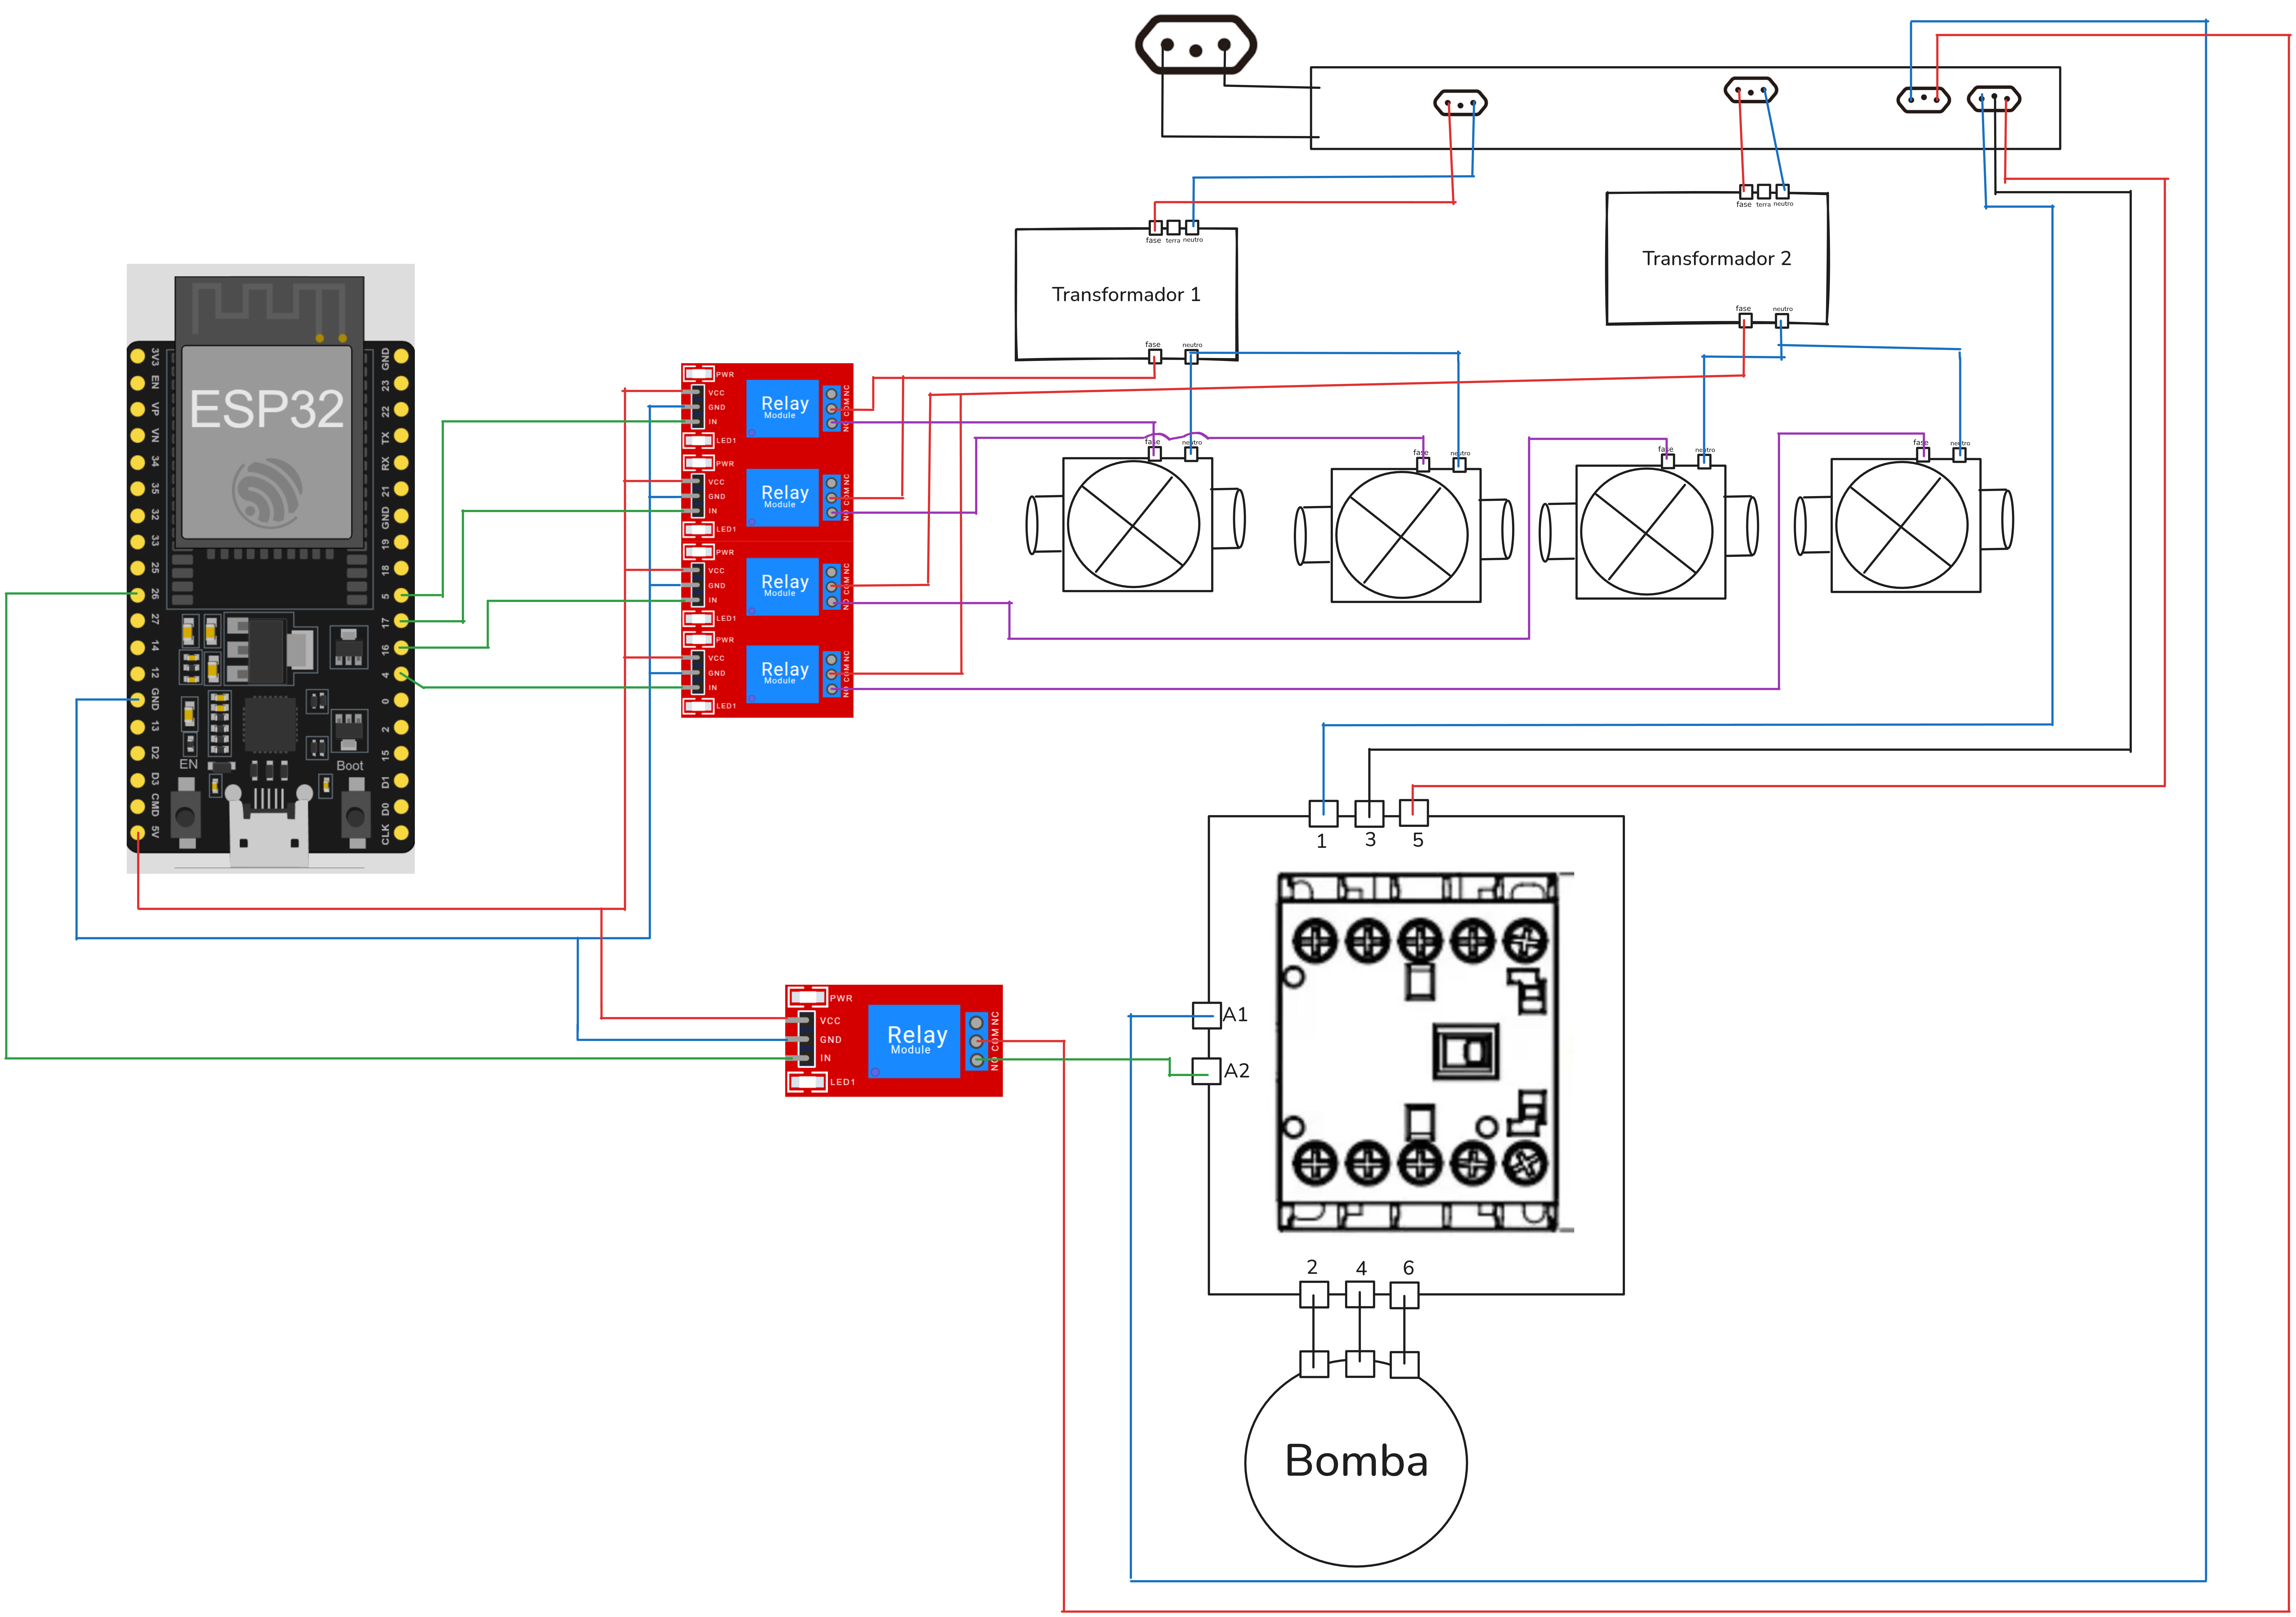
\includegraphics[width=0.8\textwidth]{circuito_2.png}
  \caption{Diagrama do circuito lógico para o sistema de irrigação.}
  \label{fig:circuito_irrigacao}
\end{figure}

\noindent\textbf{Tabela Verdade:}
A tabela verdade define ações baseadas em T (temperatura alta), U (umidade do ar baixa), S (umidade do solo baixa) e R (chuva detectada). Irrigação ocorre apenas sem chuva (R=0) e com pelo menos um indicador de seca (T, U ou S =1), modulando válvulas A-D (25-100 por cento) conforme gravidade e ativando bomba P quando necessário.
\begin{center}
\renewcommand{\arraystretch}{1.1}
\small
\begin{tabular}{|c|c|c|c||c|c|c|c|c|}
  \hline
  \textbf{T} & \textbf{U} & \textbf{S} & \textbf{R} & \textbf{A} & \textbf{B} & \textbf{C} & \textbf{D} & \textbf{P} \\
  \hline
  0 & 0 & 0 & 0 & 0 & 0 & 0 & 0 & 0 \\
  0 & 0 & 0 & 1 & 0 & 0 & 0 & 0 & 0 \\
  0 & 0 & 1 & 0 & 0 & 1 & 0 & 0 & 1 \\
  0 & 0 & 1 & 1 & 0 & 0 & 0 & 0 & 0 \\
  0 & 1 & 0 & 0 & 1 & 0 & 0 & 0 & 1 \\
  0 & 1 & 0 & 1 & 0 & 0 & 0 & 0 & 0 \\
  0 & 1 & 1 & 0 & 0 & 0 & 1 & 0 & 1 \\
  0 & 1 & 1 & 1 & 0 & 0 & 0 & 0 & 0 \\
  1 & 0 & 0 & 0 & 1 & 0 & 0 & 0 & 1 \\
  1 & 0 & 0 & 1 & 0 & 0 & 0 & 0 & 0 \\
  1 & 0 & 1 & 0 & 0 & 0 & 1 & 0 & 1 \\
  1 & 0 & 1 & 1 & 0 & 0 & 0 & 0 & 0 \\
  1 & 1 & 0 & 0 & 1 & 0 & 0 & 0 & 1 \\
  1 & 1 & 0 & 1 & 0 & 0 & 0 & 0 & 0 \\
  1 & 1 & 1 & 0 & 0 & 0 & 0 & 1 & 1 \\
  1 & 1 & 1 & 1 & 0 & 0 & 0 & 0 & 0 \\
  \hline
\end{tabular}
\end{center}

\bigskip

\noindent\textbf{O que você deve fazer:}

\begin{enumerate}[label=\textbf{\alph*)}, leftmargin=2cm]
  \item Obtenha a expressão booleana na forma canônica \textbf{Soma de Produtos (SOP)}
        para a saída da \textbf{Bomba (P)} e para todas as \textbf{Válvulas (A, B, C ou D)} 
        que possua mintermos ativos.
  \item Simplifique as funções resultantes utilizando \textbf{Álgebra Booleana},
        indicando claramente os teoremas aplicados em cada etapa.
  \item Analise o código-fonte abaixo, desenvolvido para o microcontrolador ESP32,
        que implementa a lógica booleana do sistema de irrigação. Complete a expressão
         presente após o comentário ===== RESULTADO FINAL CONSOLIDADO ===== no método processarControle() com o resultado
         das expressões simplificadas dos itens anteriores.
\end{enumerate}

\bigskip
\noindent\textbf{Código-fonte — Implementação em ESP32 (Arduino/C++):}

\begin{lstlisting}[caption={Sistema de controle de irrigação com ESP32 e sensores via API REST.}, label={lst:irrigacao_esp32}]
#include <Arduino.h>
#include <WiFi.h>
#include <HTTPClient.h>
#include <ArduinoJson.h>

// ===== CONFIG WIFI =====
const char* ssid = "SEU_WIFI";
const char* password = "SUA_SENHA";

// ===== API =====
const char* apiUrl = "http://seu-endpoint.com/api/sensores";

// ===== PINOS =====
#define PIN_A  14
#define PIN_B  27
#define PIN_C  26
#define PIN_D  25
#define PIN_P  33

// ===== VARIAVEIS =====
int T, U, S, R;

// ===== FUNCAO: LER API =====
bool lerSensoresHTTP() {
    if (WiFi.status() != WL_CONNECTED) return false;

    HTTPClient http;
    http.begin(apiUrl);

    int httpCode = http.GET();

    if (httpCode == 200) {
        String payload = http.getString();

        StaticJsonDocument<200> doc;
        DeserializationError error = deserializeJson(doc, payload);

        if (error) {
            Serial.println("Erro ao parsear JSON");
            return false;
        }

        T = doc["T"];
        U = doc["U"];
        S = doc["S"];
        R = doc["R"];

        Serial.printf("T=%d U=%d S=%d R=%d\n", T, U, S, R);

        http.end();
        return true;
    }

    http.end();
    return false;
}

// ===== FUNCAO: LOGICA BOOLEANA =====
void processarControle() {

    // ===== RESULTADO FINAL CONSOLIDADO =====
    int P = (!R) && (T || U || S);

    int A = ....
    // ===== SAIDAS =====
    digitalWrite(PIN_P, P);
    digitalWrite(PIN_A, A);
    digitalWrite(PIN_B, B);
    digitalWrite(PIN_C, C);
    digitalWrite(PIN_D, D);

    // ===== DEBUG =====
    Serial.printf("P=%d A=%d B=%d C=%d D=%d\n", P, A, B, C, D);
}

// ===== SETUP =====
void setup() {
    Serial.begin(115200);

    pinMode(PIN_A, OUTPUT);
    pinMode(PIN_B, OUTPUT);
    pinMode(PIN_C, OUTPUT);
    pinMode(PIN_D, OUTPUT);
    pinMode(PIN_P, OUTPUT);

    WiFi.begin(ssid, password);

    Serial.print("Conectando WiFi");
    while (WiFi.status() != WL_CONNECTED) {
        delay(500);
        Serial.print(".");
    }

    Serial.println("\nWiFi conectado!");
}

// ===== LOOP =====
void loop() {

    if (lerSensoresHTTP()) {
        processarControle();
    } else {
        Serial.println("Falha na leitura da API");
    }

    delay(5000); // leitura a cada 5s
}
\end{lstlisting}

\newpage
\subsection*{Exercício 3 — Piscina Olímpica}

\textbf{Contexto.}
Um condomínio possui uma piscina olímpica com sistema automatizado de controle
hidráulico. O sistema decide ativar o bombeamento para filtragem (saída $Y$)
com base em sensores industriais.

\textbf{Sensores Utilizados:}

\begin{itemize}[leftmargin=1cm, label=\textbullet]
  \item \textbf{A} — Sensor de nível ultrassônico (\textit{Siemens SITRANS Probe LU240}):\\
        $1 = $ nível adequado; $0 = $ nível baixo.
        \begin{figure}[H]
          \centering
          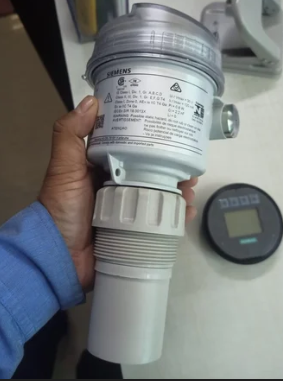
\includegraphics[width=4cm]{Siemens SITRANS Probe LU240 .png}
          \caption{Sensor de nível Siemens SITRANS Probe LU240.}
          \label{fig:siemens_level}
        \end{figure}

  \item \textbf{B} — Sensor de pressão no filtro (\textit{WIKA A-10 Pressure Transmitter}):\\
        $1 = $ pressão normal; $0 = $ pressão anormal (possível entupimento).
        \begin{figure}[H]
          \centering
          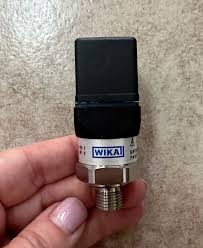
\includegraphics[width=4cm]{WIKA A-10 Pressure Transmitter .jpeg}
          \caption{Sensor de pressão WIKA A-10.}
          \label{fig:wika_pressure}
        \end{figure}

  \item \textbf{C} — Sensor de vazão na linha do dreno (\textit{Endress+Hauser Proline Promag W}):\\
        $1 = $ vazão adequada; $0 = $ sem vazão.
        \begin{figure}[H]
          \centering
          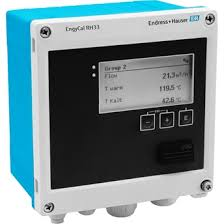
\includegraphics[width=4cm]{Endress+Hauser Proline Promag W 1.jpeg}
          \caption{Sensor de vazão Endress+Hauser Proline Promag W.}
          \label{fig:endress_vazao}
        \end{figure}

  \item \textbf{D} — Sensor de qualidade da água (\textit{Hach TU5300sc Turbidimeter}):\\
        $1 = $ água limpa; $0 = $ água turva (precisa filtrar).
        \begin{figure}[H]
          \centering
          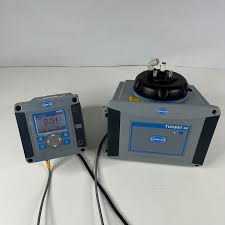
\includegraphics[width=4cm]{Hach TU5300sc Turbidimeter.jpeg}
          \caption{Turbidímetro Hach TU5300sc.}
          \label{fig:hach_turbidimeter}
        \end{figure}
\end{itemize}

\medskip
\textbf{Saída do sistema:} $Y = 1$ indica ativar bomba de filtragem; $Y = 0$ não ativar.

\bigskip

\noindent\textbf{Tabela Verdade:}

\begin{center}
\renewcommand{\arraystretch}{1.2}
\begin{tabular}{|c|c|c|c||c|}
  \hline
  \textbf{A} & \textbf{B} & \textbf{C} & \textbf{D} & \textbf{Y} \\
  \hline
  0 & 0 & 0 & 0 & \textbf{0} \\
  0 & 0 & 0 & 1 & 1 \\
  0 & 0 & 1 & 0 & 1 \\
  0 & 0 & 1 & 1 & 1 \\
  0 & 1 & 0 & 0 & 1 \\
  0 & 1 & 0 & 1 & \textbf{0} \\
  0 & 1 & 1 & 0 & 1 \\
  0 & 1 & 1 & 1 & 1 \\
  1 & 0 & 0 & 0 & 1 \\
  1 & 0 & 0 & 1 & 1 \\
  1 & 0 & 1 & 0 & \textbf{0} \\
  1 & 0 & 1 & 1 & 1 \\
  1 & 1 & 0 & 0 & 1 \\
  1 & 1 & 0 & 1 & 1 \\
  1 & 1 & 1 & 0 & 1 \\
  1 & 1 & 1 & 1 & 1 \\
  \hline
\end{tabular}
\end{center}

\bigskip

\noindent\textbf{O que você deve fazer:}

\begin{enumerate}[label=\textbf{\alph*)}, leftmargin=2cm]
  \item Obtenha a expressão booleana na forma canônica \textbf{Soma de Produtos (SOP)},
        identificando todos os mintermos onde $Y = 1$.
  \item Simplifique a função resultante utilizando as propriedades e teoremas da
        \textbf{Álgebra Booleana}. Apresente o desenvolvimento detalhado.

\item Apresente o circuíto eletrônico resultante dessa simplificação. 
\end{enumerate}



% ──────────────────────────────────────────────────────────────────────────────
\newpage
\subsection*{Exercício 4 — Controle de Catraca Industrial com Sensores IoT}

\textbf{Contexto.}
Em uma indústria, uma catraca eletrônica de acesso controla a entrada de 
funcionários em uma área restrita. O sistema utiliza sensores IoT reais para 
decidir quando liberar ou bloquear a passagem.

\textbf{Entradas (Sensores IoT):}

\begin{itemize}[leftmargin=1.5cm, label=\textbullet]
  \item \textbf{A} — Sensor RFID (\textit{leitor MFRC522}):\\
        $1 = $ cartão válido detectado; $0 = $ cartão inválido ou ausente.
  \item \textbf{B} — Sensor biométrico (\textit{R503 Fingerprint Sensor}):\\
        $1 = $ digital reconhecida; $0 = $ digital não reconhecida.
  \item \textbf{C} — Sensor de presença (\textit{HC-SR04 ultrassônico}):\\
        $1 = $ pessoa detectada na frente da catraca; $0 = $ ninguém presente.
\end{itemize}

\textbf{Saídas:}

\begin{itemize}[leftmargin=1.5cm, label=\textbullet]
  \item \textbf{X} — Liberação da catraca.
  \item \textbf{Y} — Alarme de tentativa inválida.
\end{itemize}

\bigskip

\noindent\textbf{Tabela Verdade:}

\begin{center}
\renewcommand{\arraystretch}{1.2}
\begin{tabular}{|c|c|c||c|c|}
  \hline
  \textbf{A (RFID)} & \textbf{B (Bio)} & \textbf{C (Pres)} & \textbf{X (Lib)} & \textbf{Y (Alar)} \\
  \hline
  0 & 0 & 0 & 0 & 0 \\
  0 & 0 & 1 & 0 & 1 \\
  0 & 1 & 0 & 0 & 0 \\
  0 & 1 & 1 & 1 & 0 \\
  1 & 0 & 0 & 0 & 0 \\
  1 & 0 & 1 & 1 & 0 \\
  1 & 1 & 0 & 0 & 0 \\
  1 & 1 & 1 & 1 & 0 \\
  \hline
\end{tabular}
\end{center}

\bigskip

\noindent\textbf{O que você deve fazer:}

\begin{enumerate}[label=\textbf{\alph*)}, leftmargin=2cm]
  \item Obtenha a expressão booleana na forma canônica \textbf{Soma de Produtos (SOP)}
        para as saídas \textbf{X} e \textbf{Y}.
  \item Simplifique as funções resultantes utilizando \textbf{Álgebra Booleana}. 
        Apresente as propriedades utilizadas em cada passo.
\end{enumerate}


% ──────────────────────────────────────────────────────────────────────────────
\newpage
\subsection*{Exercício 5 — Sistema Inteligente para Tanque de Tilápia}

\textbf{Contexto.}
Um sistema de monitoramento de um tanque de tilápia utiliza sensores IoT 
industriais para decidir quando ativar o sistema de renovação de água ($R$).

\textbf{Entradas (Sensores):}

\begin{itemize}[leftmargin=1.5cm, label=\textbullet]
  \item \textbf{D} — Sensor de oxigênio dissolvido ($1 = $ baixo oxigênio; $0 = $ adequado).
  \item \textbf{T} — Sensor de temperatura ($1 = $ temperatura alta; $0 = $ ideal).
  \item \textbf{N} — Sensor de amônia ($1 = $ alta concentração; $0 = $ segura).
\end{itemize}

\textbf{Saída:}

\begin{itemize}[leftmargin=1.5cm, label=\textbullet]
  \item \textbf{R} — Sistema de renovação de água ($1 = $ ativado; $0 = $ desligado).
\end{itemize}

\bigskip

\noindent\textbf{Tabela Verdade:}

\begin{center}
\renewcommand{\arraystretch}{1.2}
\begin{tabular}{|c|c|c||c|}
  \hline
  \textbf{D} & \textbf{T} & \textbf{N} & \textbf{R} \\
  \hline
  0 & 0 & 0 & 0 \\
  0 & 0 & 1 & 1 \\
  0 & 1 & 0 & 1 \\
  0 & 1 & 1 & 0 \\
  1 & 0 & 0 & 1 \\
  1 & 0 & 1 & 0 \\
  1 & 1 & 0 & 1 \\
  1 & 1 & 1 & 1 \\
  \hline
\end{tabular}
\end{center}

\bigskip

\noindent\textbf{O que você deve fazer:}

\begin{enumerate}[label=\textbf{\alph*)}, leftmargin=2cm]
  \item Obtenha a expressão booleana canônica \textbf{Soma de Produtos (SOP)} 
        da saída \textbf{R}, a partir da tabela verdade.
  \item Realize a simplificação da expressão utilizando \textbf{Álgebra Booleana}.
  \item Apresente o circuíto digital utilizando portas lógicas para a(s) saída(s).
\end{enumerate}

\end{document}
